%%%%%%%%%%%%%%%%%%%%%%%%%%%%%%%%%%%%%%%%%%%%%%%%%%%%%%%
%
%                                                       Example IS Template
%
% \documentclass{woosterthesis} must be at the beginning of every IS. Options are the same as
% for the report class with some additional options, abstractonly, blacklinks, code, kaukecopyright, palatino, picins,
% maple, index, verbatim, dropcaps, euler, gauss, alltt,  woolshort, colophon, woosterchicago, and
% achemso. The kaukecopyright option will put the arch symbol with the word mark on the
% copyright page. The woosterthesis class is based on the report class. One thing to note is that
% the ``%'' symbol comments out all characters that follow it on the line.
%
%%%%%%%%%%%%%%%%%%%%%%%%%%%%%%%%%%%%%%%%%%%%%%%%%%%%%%%

%%%%%%%%%%%%%%%%%%%%%%%%%%%%%%%%%%%%%%%%%%%%%%%%%%%%%%%
% use this declaration for a draft version of your IS
\documentclass[10pt,palatino,code,picins,kaukecopyright,openright,woolshort,dropcaps,verbatim,index,euler]{woosterthesis}
%\documentclass[10pt,code,picins,kaukecopyright,openright,woolshort,dropcaps,verbatim,euler,index,colophon,blacklinks,twoside]{woosterthesis}
% note that you can specify the woosterchicago option to use Chicago citation style and achemso to use the American Chemical Society citation format
%
%%%%%%%%%%%%%%%%%%%%%%%%%%%%%%%%%%%%%%%%%%%%%%%%%%%%%%%
%
% use this declaration for the print version of your IS
%\documentclass[12pt,code,palatino,picins,blacklinks,kaukecopyright,openright,twoside]{woosterthesis} % probably what most students would use
%
%%%%%%%%%%%%%%%%%%%%%%%%%%%%%%%%%%%%%%%%%%%%%%%%%%%%%%%
%
% use this declaration for the PDF version of your IS
%\documentclass[12pt,code,palatino,picins,kaukecopyright,openright,twoside]{woosterthesis}
%
%%%%%%%%%%%%%%%%%%%%%%%%%%%%%%%%%%%%%%%%%%%%%%%%%%%%%%%

%%%%%%%%%%%%%%%%%%%%%%%%%%%%%%%%%%%%%%%%%%%%%%%%%%%%%%%
%
%                                                       Load Packages
%
%   To load packages in addition to the ones that are loaded by default, please place your
%   usepackage commands in the packages.tex file in the styles folder.
%
%%%%%%%%%%%%%%%%%%%%%%%%%%%%%%%%%%%%%%%%%%%%%%%%%%%%%%%

%%%%%%%%%%%%%%%%%%%%%%%%%%%%%%%%%%%%%%%%%%%%%%%%%%%%%%%%%%%%%%%%%%%%%%%%%%%%%%%%%%%%%%%%%%%%%%
%
%                                                       Packages
%
% Do not add any other packages without consulting with Dr. Breitenbucher as they may break the functionality of the class.
%
%%%%%%%%%%%%%%%%%%%%%%%%%%%%%%%%%%%%%%%%%%%%%%%%%%%%%%%%%%%%%%%%%%%%%%%%%%%%%%%%%%%%%%%%%%%%%%

\ifxetex%
	\defaultfontfeatures{Mapping=tex-text}%
		\setmainfont[Numbers=OldStyle,BoldFont={* Semibold}]{Adobe Garamond Pro}% select the body font other choices would be Baskerville, Optima Regular, Didot, Georgia, Cochin
                      \setmathrm{Adobe Garamond Pro}
                      \setmathfont[Digits,Latin]{Adobe Garamond Pro}
		\setsansfont[Scale=.87,Fractions=On,Numbers=Lining]{Myriad Pro}% select the sans serif font other choices would be Skia, Arial, Helvetica, Helvetica Neue
%		\setmonofont[Scale=.88,Fractions=On]{Prestige Elite Std Bold}% set the mono font other choices would be Courier, Monaco, American Typewriter
	           \setmonofont[Scale=.9]{Courier Std}%
%	    \setromanfont[Fractions=On,Numbers=OldStyle, BoldFont={Warnock Pro Semibold}]{Warnock Pro}%
%	    \setsansfont[Scale=.95,Fractions=On,Numbers=Lining]{Myriad Pro}%
%	    \setmonofont[Scale=.91,Fractions=On]{Courier Std Medium}%
%	    \setmonofont[Scale=.88,Fractions=On]{American Typewriter}%
%		\setmonofont[Scale=.94,Fractions=On]{Prestige Elite Std Bold}
%    		\setromanfont[Fractions=On,Numbers=OldStyle]{Minion Pro}
 %    	\setsansfont[Scale=.9,Fractions=On,Numbers=Lining]{Myriad Pro}
%     	\setmonofont[Scale=.93,Fractions=On]{Courier Std Medium}
%     	\setromanfont[Fractions=On,Numbers=OldStyle]{Minion Pro}
%     	\setsansfont[Scale=.85,Fractions=On,Numbers=Lining]{News Gothic Std}
%    		\setmonofont[Scale=.93,Fractions=On]{Prestige Elite Std}
%		\setromanfont[Fractions=On,Numbers=OldStyle]{Minion Pro}
%		\setsansfont[Scale=.9,Fractions=On,Numbers=Lining]{Bell Gothic Std Bold}
%		\setmonofont[Scale=.95,Fractions=On]{Prestige Elite Std Bold}
\fi
\usepackage{mathtools}
\newtheorem{define}{Definition}
\usepackage{amssymb}
\usepackage{graphicx}

%%%%%%%%%%%%%%%%%%%%%%%%%%%%%%%%%%%%%%%%%%%%%%%%%%%%%%%
%
%                                                       Load Personal commands
%                                                                    
%  There will be certain commands that you use frequently in the thesis. You can give these
%  commands new names which are easier for you to remember. You can also combine several
%  commands into a new command of your own. See The LaTeX Companion or Guide to LaTeX
%  for examples on defining your own commands. These are commands that I defined to cut
%  down on typing. You can enter your commands in the personal.tex file in the styles folder.
%
%%%%%%%%%%%%%%%%%%%%%%%%%%%%%%%%%%%%%%%%%%%%%%%%%%%%%%%

%%%%%%%%%%%%%%%%%%%%%%%%%%%%%%%%%%%%%%%%%%%%%%%%%%%%%%%%%%%%%%%%%%%%%%%%%%%%%%%%%%%%%%%%%%%%%%
%
%                                                       Personal Commands
%                                                                    
% There will be certain commands that you use frequently in the thesis. You can give these
% commands new names which are easier for you to remember. You can also combine several
% commands into a new command of your own. See The LaTeX Companion or Guide to LaTeX for
% examples on defining your own commands. These are commands that I defined to cut down on typing.
%
%%%%%%%%%%%%%%%%%%%%%%%%%%%%%%%%%%%%%%%%%%%%%%%%%%%%%%%%%%%%%%%%%%%%%%%%%%%%%%%%%%%%%%%%%%%%%%

\newcommand{\fl}{\ell}
\newcommand{\lt}{\LaTeX\ }
\newcommand{\msw}{Word\texttrademark\ }
\newcommand{\xt}{\ifthenelse{\boolean{xetex}}{\XeTeX\ }{XeTeX} }
%\newcommand{\Cl}{\ensuremath{\textup{C}_\fl}}
%\newcommand{\bCl}{C$_{\ell}$}
%\newcommand{\Al}{\ensuremath{\textup{A}_\fl}}
%\newcommand{\msum}{{(m_1+\cdots+m_\ell)}}
%\newcommand{\Nsum}{{(N_1+\cdots+N_\ell)}}
%\newcommand{\ysum}{{(y_1+\cdots+y_\ell)}}
%\newcommand{\Nsub}{{N_1+\cdots+N_\ell}}
%\newcommand{\ysub}{{y_1+\cdots+y_\ell}}
%\newcommand{\xsub}{{x_1+\cdots+x_\ell}}
%\newcommand{\ysqsum}{{y_1^2+\cdots +y_{\fl}^2}}
%\newcommand{\msqsum}{{m_1^2+\cdots +m_{\fl}^2}}
%\newcommand{\ratio}{\left(\frac{\beta}{\alpha}\right)}
%\newcommand{\LT}{\ensuremath{\LaTeX{}}}

%%%%%%%%%%%%%%%%%%%%%%%%%%%%%%%%%%%%%%%%%%%%%%%%%%%%%%%%%%%%%%%%%%%%%%%%%%%%%%%%%%%%%%%%%%%%%%
% These commands have one argument and are entered as \commandname{argument}.
%%%%%%%%%%%%%%%%%%%%%%%%%%%%%%%%%%%%%%%%%%%%%%%%%%%%%%%%%%%%%%%%%%%%%%%%%%%%%%%%%%%%%%%%%%%%%%

%\newcommand{\bd}[1]{\textbf{#1}}
\newcommand{\mbd}[1]{{\mathbf{#1}}}
%\newcommand{\abs}[1]{\vert{#1}\vert}
\newcommand{\bvec}[1]{{\mbd{#1}}}
%\newcommand{\lvec}[1]{\abs{\bvec{#1}}}
%\newcommand{\nesmallprod}[1]{\prod_{\substack{#1=1\\
%#1\neq p}}^{\fl}}
%\newcommand{\esec}[1]{e_{2}({#1}_1,\ldots ,{#1}_\fl)}
%\newcommand{\smallprod}[1]{\prod_{#1=1}^{\fl}}
%\newcommand{\incsum}[1]{{#1}_2+2{#1}_3+\cdots +(\fl -1){#1}_\fl}
%\newcommand{\binomsum}[1]{\binom{{#1}_1}{2}+\cdots +\binom{{#1}_\fl}{2}}
%\newcommand{\imultsum}[1]{\multsum{{#1}_k\ge 0}{k=1,\ldots ,\fl}}
%\newcommand{\diagsum}[1]{\sum _{\substack{{#1}_k\ge 0\\
%k=1, \ldots ,\fl\\
%\lvec{#1}=m}}}
%\newcommand{\Mb}[1][\fl]{\ensuremath{\textup{\bd{M}}_b^{(#1)}}}
%\newcommand{\HLV}[1]{\ensuremath{\textup{\bd{H}}_{#1}}}
%\newcommand{\Rq}[1][p]{\ensuremath{\textup{R}_q^{(#1)}}}
\newcommand{\degree}[1]{\ensuremath{#1^{\circ}}}
\newcommand{\ip}[1]{\texttt{#1}\index{packages!#1}}
\newcommand{\ic}[1]{\texttt{$\backslash$#1}\index{commands!#1}}
\newcommand{\ie}[1]{#1\index{#1}}

%%%%%%%%%%%%%%%%%%%%%%%%%%%%%%%%%%%%%%%%%%%%%%%%%%%%%%%%%%%%%%%%%%%%%%%%%%%%%%%%%%%%%%%%%%%%%%
% These commands have 2 or more arguments some with default values for the first argument. You
% can learn a lot about constructing complicated equations by studying the commands in this %section.
%%%%%%%%%%%%%%%%%%%%%%%%%%%%%%%%%%%%%%%%%%%%%%%%%%%%%%%%%%%%%%%%%%%%%%%%%%%%%%%%%%%%%%%%%%%%%%

%\newcommand{\qbinom}[2]{\ensuremath{\left[{#1}\atop{#2}\right]_q}}
%\newcommand{\sqprod}[2]{\prod_{#1,#2=1}^{\fl}}
%\newcommand{\triprod}[2]{\prod_{1\le #1<#2\le \fl}}
%\newcommand{\nesqprod}[2]{\prod_{\substack{#1,#2=1\\
%#1,#2\neq p}}^{\fl}}
%\newcommand{\netriprod}[2]{\prod_{\substack{1\le #1<#2\le \fl\\
%#1,#2\neq p}}}
\newcommand{\qrfac}[3][\ ]{\left({#2}\right)_{#3}^{#1}}
%\newcommand{\multsum}[2]{\sum_{\substack{{#1}\\
%\\
%{#2}}}}
%\newcommand{\fmultsum}[2][N]{\multsum{0\le {{#2}_k}\le {{#1}_k}}{k=1,\ldots ,\fl}}
%\newcommand{\pq}[2]{\ _{#1}\varphi_{#2}}
%\newcommand{\mess}[2][y_k]{\frac{\qrfac{\alpha x_k}{#2}\qrfac{qx_k\beta^{-1}}{#2}}{\qrfac{\beta x_k}{#1}
%\qrfac{qx_k\alpha^{-1}}{#1}}}
%\newcommand{\MG}[7][\fl]{\ensuremath{\left[\textup{MG}\right]_{#2}^{(#1)}{#3}q;{#4};{#5}^{#6}{#7}}}

%%%%%%%%%%%%%%%%%%%%%%%%%%%%%%%%%%%%%%%%%%%%%%%%%%%%%%%%%%%%%%%%%%%%%%%%%%%%%%%%%%%%%%%%%%%%%%
% These commands define new environments
%%%%%%%%%%%%%%%%%%%%%%%%%%%%%%%%%%%%%%%%%%%%%%%%%%%%%%%%%%%%%%%%%%%%%%%%%%%%%%%%%%%%%%%%%%%%%%

\newcounter{unnumft}
\setcounter{unnumft}{0}
\newenvironment{unnumft}[2]{\renewcommand{\thefootnote}{}\footnote{#1}\footnote{#2}} {\addtocounter{footnote}{-2}}
\newenvironment{wooexample}{\small
\begin{singlespace}
\begin{example}}{\end{example}
\end{singlespace}}

\graphicspath{{./figures/}}% for setting where to look for figures
\citestyle{wooster}% change the style of citations. Math and CS people should leave this alone.






%%%%%%%%%%%%%%%%%%%%%%%%%%%%%%%%%%%%%%%%%%%%%%%%%%%%%%%
%
%                                                       Load Theorem formatting information
%
%  If you need to define an new theorem style or want to see what theorem like environments 
%  are available please look at the theorems.tex file in the styles folder.
%
%%%%%%%%%%%%%%%%%%%%%%%%%%%%%%%%%%%%%%%%%%%%%%%%%%%%%%%

%%%%%%%%%%%%%%%%%%%%%%%%%%%%%%%%%%%%%%%%%%%%%%%%%%%%%%%%%%%%%%%%%%%%%%%%%%%%%%%%%%%%%%%%%%%%%%
%
% This is where one would tell \LaTeX{} how to format Theorems, Definitions, etc. and also
% indicate the environment names. You need the amsthm package (loaded in the woosterthesis %class) in order for these commands to work.
%
%%%%%%%%%%%%%%%%%%%%%%%%%%%%%%%%%%%%%%%%%%%%%%%%%%%%%%%%%%%%%%%%%%%%%%%%%%%%%%%%%%%%%%%%%%%%%%

% an example of defining your own theoremstyle
%\newtheoremstyle{break}% name
%  {\topsep}%      Space above
%  {\topsep}%      Space below
%  {\itshape}%         Body font
%  {}%         Indent amount (empty = no indent, \parindent = para indent)
%  {\bfseries}% Thm head font
%  {.}%        Punctuation after thm head
%  {\newline}%     Space after thm head: " " = normal interword space;
%        %       \newline = linebreak
%  {}%         Thm head spec (can be left empty, meaning `normal')
\newtheoremstyle{scthm}{\topsep}{\topsep}{\itshape}{}{\bfseries\scshape}{}{ }{}% small cap font for the heading
\newtheoremstyle{itdefn}{\topsep}{\topsep}{\itshape}{}{\bfseries}{.}{ }{}% italic definitions
\newtheoremstyle{scdefn}{\topsep}{\topsep}{\itshape}{}{}{}{ }{\thmname{\textbf{#1}}\thmnumber{ \textbf{#2}}\thmnote{ \scshape #3:}}% small cap headings and italic text.

\theoremstyle{break}% this theoremstyle will put the text of the theorem on a new line.
\newtheorem{thm}{Theorem}[chapter]%number theorems within chapters 
%\newtheorem{cor}[thm]{Corollary}%by using [thm] we are numbering these environments with the theorems.
\newtheorem{cor}{Corollary}[chapter]%number corollaries within chapters .
%\newtheorem{lem}[thm]{Lemma}
\newtheorem{lem}{Lemma}[chapter]
%\newtheorem{prop}[thm]{Proposition}
\newtheorem{prop}{Proposition}[chapter]

\theoremstyle{scdefn}
%\newtheorem{defn}[thm]{Definition}
\newtheorem{defn}{Definition}[chapter]
\theoremstyle{remark}
%\newtheorem{rem}[thm]{Remark}
\newtheorem{rem}{Remark}[chapter]
\renewcommand{\therem}{}
%\newtheorem{ex}[thm]{Example}
\newtheorem{ex}{Example}[chapter]

\theoremstyle{plain}
%\newtheorem{note}[thm]{Notation}
\newtheorem{note}{Notation}[chapter]
\renewcommand{\thenote}{}
%\newtheorem{nts}[thm]{Note to self}%use to remind yourself of things yet to do
\newtheorem{nts}{Note to self}[chapter]
\renewcommand{\thents}{}
%\newtheorem{terminology}[thm]{Terminology}
\newtheorem{terminology}{Terminology}[chapter]
\renewcommand{\theterminology}{}

\theoremstyle{itdefn}
\newtheorem{bdefn}{Definition}[chapter]
\newsavebox{\fmbox} 
\newenvironment{boxeddefn}[2] 
{\begin{lrbox}{\fmbox}\begin{minipage}{0.9 \linewidth }\begin{singlespace}\begin{bdefn}[{#1}]\label{#2}\vspace{0.2cm}} 
{\end{bdefn}\end{singlespace}\end{minipage}\end{lrbox}\fbox{\usebox{\fmbox}}}

\setcounter{secnumdepth}{5}% controls the numbering of sections
\setcounter{tocdepth}{6}% controls the number of levels in the Contents

%%%%%%%%%%%%%%%%%%%%%%%%%%%%%%%%%%%%%%%%%%%%%%%%%%%%%%%
%
%  This is where one enters the information about the thesis.
%
%%%%%%%%%%%%%%%%%%%%%%%%%%%%%%%%%%%%%%%%%%%%%%%%%%%%%%%


\title{Game Theory and AI in Video Game Enemies}
\thesistype{} % you should make this Independent Study Thesis
\author{Nicholas Czaban}
%\presentdegrees{Ph.D.} % you should comment this line
\degreetoobtain{Your degree}
\presentschool{The College of Wooster}
\academicprogram{Computer Science and Mathematics}
\gradyear{2019}
\advisor{Dr. Denise Byrnes (Computer Science)}
\secondadvisor{Dr. Pamela Pierce (Mathematics)}
%\reader{Reader}
\copyrighted   
%\copyrightdate{}                  
\makeindex % comment this line if you do not have an index

%%%%%%%%%%%%%%%%%%%%%%%%%%%%%%%%%%%%%%%%%%%%%%%%%%%%%%%
%
%  This is where the commands for the document begin. All \LaTeX{} documents must have a
%  \begin{document} text .... \end{document} structure.
%
%%%%%%%%%%%%%%%%%%%%%%%%%%%%%%%%%%%%%%%%%%%%%%%%%%%%%%%

\begin{document}

%%%%%%%%%%%%%%%%%%%%%%%%%%%%%%%%%%%%%%%%%%%%%%%%%%%%%%%
%
%  The front matter includes acknowledgments, dedications, vitas, list of tables, list of figures,
%  copyright, abstract, title page, and contents.
%
%%%%%%%%%%%%%%%%%%%%%%%%%%%%%%%%%%%%%%%%%%%%%%%%%%%%%%%

\frontmatter
\maketitle
\ClearShipoutPicture
\clearpage\thispagestyle{empty}\null\clearpage
\disscopyright 

%%%%%%%%%%%%%%%%%%%%%%%%%%%%%%%%%%%%%%%%%%%%%%%%%%%%%%%
%                                                                                       
%                                                       Abstract						
%                                                                                       
%%%%%%%%%%%%%%%%%%%%%%%%%%%%%%%%%%%%%%%%%%%%%%%%%%%%%%%

\begin{abstract}

\end{abstract}

%%%%%%%%%%%%%%%%%%%%%%%%%%%%%%%%%%%%%%%%%%%%%%%%%%%%%%%
%                                                                                       
%                                                       Dedications					
%                                                                                       
%%%%%%%%%%%%%%%%%%%%%%%%%%%%%%%%%%%%%%%%%%%%%%%%%%%%%%%

\dedication{}


%%%%%%%%%%%%%%%%%%%%%%%%%%%%%%%%%%%%%%%%%%%%%%%%%%%%%%%
%                                                                                       
%                                                       Acknowledgments					
%                                                                                       
%%%%%%%%%%%%%%%%%%%%%%%%%%%%%%%%%%%%%%%%%%%%%%%%%%%%%%%

\begin{acknowl}

\end{acknowl}

%%%%%%%%%%%%%%%%%%%%%%%%%%%%%%%%%%%%%%%%%%%%%%%%%%%%%%%
%                                                                                       
%                                                       Vita					
%                                                                                       
%%%%%%%%%%%%%%%%%%%%%%%%%%%%%%%%%%%%%%%%%%%%%%%%%%%%%%%

%\begin{vita} 
% You talk about yourself and how you got to where you are now. There is a structured form for the Vita that can be used if you want, but I don't encourage it.

%%%%%%%%%%%%%%%%%%%%%%%%%%%%%%%%%%%%%%%%%%%%%%%%%%%%%%%
%
%  The list below is for a thesis that requires a more structured Vita such as a masters or Ph.D.
%
%%%%%%%%%%%%%%%%%%%%%%%%%%%%%%%%%%%%%%%%%%%%%%%%%%%%%%%

%\begin{datelist}
%\item[April 6, 1970]Born-Wooster, Ohio
%\item[August 11, 1990]Chosen to present an undergraduate paper at the 75th meeting of the MAA, Columbus, Ohio
%\item[August 1990--August 1991]President Wooster Student Chapter of the MAA, The College of Wooster, Wooster, Ohio
%\item[August 1991--May 1992]Secretary Wooster Student Chapter of the MAA, The College of Wooster, Wooster, Ohio
%\item[1992]\emph{Phi Beta Kappa} (on junior standing), The College of Wooster, Wooster, Ohio
%\item[1992]Elizabeth Sidwell Wagner Prize in Mathematics, The College of Wooster
%\item[1992]William H. Wilson Prize in Mathematics, The College of Wooster
%\item[May 11, 1992]B.A., Mathematics, The College of Wooster
%\item[1997]Finalist for Graduate Teaching Award, The Ohio State University, Columbus, Ohio
%\item[June 21-25, 1998]Participant in the AMS-IMS-SIAM Summer Research Conferences: q-Series, Combinatorics, and Computer Algebra, Mt. Holyoke, Massachusetts
%\item[October 1998--October 1999]Graduate student representative to The Ohio State University Department of Mathematics Graduate Studies Committee, Columbus, Ohio
%\item[January 1999]q-series seminar address, The Ohio State University, Columbus, Ohio
%\item[2000]Finalist for Departmental Teaching Award, The Ohio State University, Columbus, Ohio
%\item[2000]Nominated for Graduate Teaching Award, The Ohio State University, Columbus, Ohio
%\item[April 2000]Invited colloquium talk at The College of Wooster, Wooster, Ohio
%\item[1992-- present]Graduate Teaching and Research Associate, The Ohio State University
%\end{datelist}
%
%%%This is for any publications you might have.%%%%%

%\begin{publist}  
%\pubitem{\quad}
%\pubitem{\quad}
%\end{publist} 

%\begin{fieldsstudy} 
%    \majorfield{Major}
%	\minorfield{Minor}
%    \specialization{Area of IS research}
    %\begin{studieslist}
   %\studyitem{Abstract Algebra}{Hampton}
   %\end{studieslist}
%  \end{fieldsstudy}
%\end{vita}

%%%%%%%%%%%%%%%%%%%%%%%%%%%%%%%%%%%%%%%%%%%%%%%%%%%%%%%
%
%  We now create the contents page and if necessary the list of figures and list of tables.
%
%%%%%%%%%%%%%%%%%%%%%%%%%%%%%%%%%%%%%%%%%%%%%%%%%%%%%%%


\cleardoublepage
\phantomsection
\addcontentsline{toc}{chapter}{Contents}

\tableofcontents
%\listoffigures %Use if you have a list of figures.
%\listoftables %Use if you have a list of tables.
%\lstlistoflistings %Use if you are using the code option

%%%%%%%%%%%%%%%%%%%%%%%%%%%%%%%%%%%%%%%%%%%%%%%%%%%%%%%

%\input{chapters/preface} % most theses do not have a preface so this should be commented

%%%%%%%%%%%%%%%%%%%%%%%%%%%%%%%%%%%%%%%%%%%%%%%%%%%%%%%
\mainmatter

%%%%%%%%%%%%%%%%%%%%%%%%%%%%%%%%%%%%%%%%%%%%%%%%%%%%%%%
%
%                                                       Thesis Chapters
%
% This is where the main text of the thesis goes. I have written this template assuming that
% each chapter is a separate file. You do not have to do this but it makes things easier to find
% for editing. You can use the sample chapters to help you figure out how to type things into
% your thesis. To include a chapter just use the \include{chaptername} command. Chapters are
% included in the order listed.
%
%%%%%%%%%%%%%%%%%%%%%%%%%%%%%%%%%%%%%%%%%%%%%%%%%%%%%%%

%\input{chapters/introduction}
%\section{Extensive-Form Game Trees}
%The quintessential example of Game Theory, the prisoner's dilemma, expresses the possible outcomes in a matrix form. Both players have two possible choices, resulting in the 2x2 matrix. However, for games with sequential actions or numerous choices, the matrix representation quickly becomes unreadable. Thus, games where players take turns performing actions are represented in extensive- or tree-form. In these trees, each node is a possible choice for one of the players, and the edges are the actions that they can take for that choice. At the leaves of this tree are the results of each player's utility function\cite{shoh09}.\\

%Specifically, these trees are most useful for perfect-information, constant-sum games. For a game to be perfect-information, each player must know the series of actions that led to a particular node. In contrast, imperfect-information games have nodes which are indistinguishable from other nodes, at least with the information available to a player \cite{shoh09}. Consider a game where a player picks between three doors, one of which has a reward behind it. For multiple rounds of this game, the player has no way of knowing which door has the prize; thus, any choice node for that player is indistinguishable from another and no pure strategy exists. In constant-sum games, any gain one player makes to their utility function causes a constant value loss in another player's utility function. This behavior is expressed as $\forall a\in A_1\times A_2, u_1(a)+u_2(a) = c$ where $a$ is a strategy profile in sets of actions $A_1,A_2$ for players 1 and 2 and $u_1,u_2$ are the utility functions for these players. For convenience, $u$ is often set as 0, meaning that any positive action by one player causes an equivalent loss in the other player. These cases are referred to as zero-sum games \cite{schw04}. Certain nonzero-sum games, such as Monopoly, can be represented as zero-sum games if the ``board'' (or the bank, as in Monopoly) is treated as a player. Thus, two players forming an alliance would be working against this nonexistent player, and all properties of zero-sum games can be applied.\\

%In these game trees, the first player to make a choice is referred to as \textbf{max} and the second player as \textbf{min}. A choice for a particular player is thus referred to as either a max-node or a min-node, depending on the turn. Another crucial concept is \textit{ply}, the number of actions required to travel from one node to another \cite{smed06}. When a game is expressed in this form, it is trivial to see which move will be taken one ply above the leaves: if player \textbf{max} can win, they will take the action that leads to their victory; if they cannot win, they will try to reach a draw if possible. With this idea in mind, the strategy for additional plys above the leaves can be determined recursively.\\

%It was proven that any decision tree of this type can be represented as a collection of sets ordered by set inclusion, without loss of generality \cite{alos08}. This definition of a ``set-tree'' is able to encompass numerous types of games. These include stochastic games, where the environment of the game changes with a player's decision \cite{sola15}; repeated games, where the incentives of a repeated interaction differs from an isolated interaction \cite{mail06}; and differential games, where players make continuous decisions \cite{alos08}. There are two desired traits for these game trees: every strategy or combination of actions produces an outcome, and the outcome of a particular strategy is unique \cite{alos08}. If an extensive-form game has these qualities, then the game can also be expressed in normal form; these traits are necessary and sufficient for normal-form representation.


%\section{Pygame and Game Design}
%The example Pygame files create classes for each entity in the game (alien, player, projectile, scoreboard) and has one main loop. These classes contain elements such as speed, their sprite images, and \_\_init\_\_ and update functions. The main loop is fairly iterative, but there does not seem to be any restriction on doing things more functionally.

\chapter{Introduction}
% !TEX root = ../IS.tex
\chapter{Extensive Form Games}
\section{Basics of Game Theory}
Frequently used, and originally explored in economic contexts, game theory is the study of interactions between decision-makers. Antoine Cournot attempted to explain the decisions of duopolies (markets with only two sellers producing a product) in 1838 using the concept of strategic behavior \cite{webs14}. In this case, strategic behavior refers to scenarios where one person's decisions both affect and are affected by the decisions of other persons. Cournot later influenced Joseph Bertrand's 1883 work, which examined strategic decisions in product pricing. These early efforts were limited by standard economic methodologies; it wasn't until John von Neumann's 1928 proof of the minimax theorem and his later collaboration with economist Oskar Morgenstern that the modern field of game theory began \cite{webs14}. The strategies involved with game theory are used to explain collusion and subsequent breakdown of oligopolies like OPEC, and the symbiosis between sharks and pilot fish.\\

As we begin our study of game theory, it is important to precisely define what games are. A game is defined as an interaction constraining the actions a player can perform and the interests of players; Game theory involves the techniques used to analyze and determine solutions and outcomes of various games \cite{osbo94}. It is assumed that players in these games are both rational (they pursue well-defined objectives, generally in their own self-interest) and strategic (they take the knowledge and behavior of other decision-makers into account)\cite{osbo94}.\\

The goals of these players are represented using a utility function. In game theory, utility is the quantitative measure of a choice's value; this could be a monetary value or it could be expressed in terms of the happiness a player gains from that outcome, depending on the structure of the ``game''. A highly desired outcome for a player will have a higher utility than an undesirable outcome. Utility is the core of ``zero-sum games.'' In these games, one player's increase in utility corresponds to another player's equal loss in utility. For example, a player might earn \$5 in a zero-sum game by directly taking those \$5 from another player.

\section{Normal Form Games}
In the vast majority of human choices, a person will attempt to maximize their utility function; they will perform actions that benefit themselves. When there are two or more agents trying to maximize their utility, the interactions and choices between these agents, or players, become more and more complex. These interactions can be studied with game theory using the normal or strategic form.
\begin{define}
  A finite normal-form game is a tuple $(N, A, u)$ where:
  \begin{itemize}
  \item $N$ is a finite set of $n$ players, indexed by $i$
  \item $A=A_1\times\cdots\times A_n$, where $A_i$ is a finite set of actions available to player $i$. Each vector $a=(a_1,\cdots ,a_n)\in A$ is called an action profile.
    \item $u=(u_1,\cdots ,u_n)$ where $u_i : A \mapsto\mathbb{R}$ is a real-valued utility function for player $i$. \cite{shoh09}
\end{itemize}
\end{define}

In an arbitrary normal-form game, there are $n$ different players contained in the set $N$, where $n$ is a positive integer. For each of these players, there is also a finite set of actions that they can take. Player $N_i$ will have the action set $A_i$. The complete action set $A$ is determined by the Cartesian product of the action sets of each player. Within $A$, a vector $a$ is the action profile; an action profile, or outcome, represents the choice that each player makes \cite{osbo94}. The collection of mappings $u$ gives each action profile a particular value; these values determine which outcome is preferred by a player. In normal-form games, players are utility-maximizing agents; they will gravitate towards action profiles that give them higher utility.\\

An example of a normal-form game can be seen in the quintessential ``Prisoner's Dilemma'' example. This game is expressed in a 2x2 matrix, with one player's choices represented in the columns and the other player's choices represented in the rows of said matrix.

\begin{figure}[H]
  \centering
  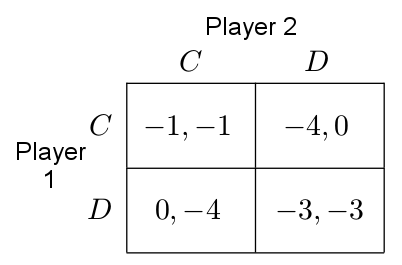
\includegraphics[width=7cm]{figures/ExampleGrid.png}
  \caption{The Prisoner's Dilemma, represented in a normal form matrix \cite{shoh09}.}
  \label{fig:prisoner}
\end{figure}

In Figure \ref{fig:prisoner}, the column labeled \textit{C} represents prisoner 2 cooperating with their partner, while the column labeled \textit{D} represents prisoner 2 defecting, telling the police that their partner is guilty. The rows \textit{C} and \textit{D} represent the same choices for prisoner 1. For this game, $A_i$ would be the set $\{C, D\}$, as those are the two choices that each prisoner can make. Thus, $A=A_1\times A_2 = \{(C, C), (C, D), (D, C), (D, D)\}$, or all four possible outcomes for this game. An action profile $a$ in this game would then be any of the ordered pairs in $A$; $(C,D)$, for instance, is an action profile. The ordered pairs of the matrix represent the values of each player's respective utility function in that outcome. In this case, their utility is the number of years in jail to which a player is sentenced. The mapping functions in $u$ correspond to the leniency of the courts; unfortunately, the quantitative functions in $u$ that the courts use in this example are unknown, and only the values at these specific points are known. When both prisoners cooperate, they both get one year in prison; their sentence is lighter without their confession. If only one prisoner confesses, that player gets off with not prison, while the other player gets four years in jail. If both prisoners rat out their partner for committing the crime, both prisoners get three years in prison.\\

From the perspective of an individual player, they must consider their options before proceeding. The best strategy of a player would be trivial if that player also knew which strategies the other player(s) were adopting \cite{shoh09}. This would be a \textit{pure strategy} option, where the player selects a single action and always that action. However, in the prisoner's dilemma, the two are being interrogated separately, and one player does not know the other player's choice. Thus, the prisoners must create a \textit{mixed strategy} by introducing probability to their decisions.

\begin{define}
  Let $(N,A,u)$ be a normal-form game, and for any set $X$ let $\Pi(X)$ be the set of all probability distributions over $X$. The set of mixed strategies for player $i$ is $S_i = \Pi(A_i)$, and the probability an action $a_i\in A_i$ will be played is denoted $s_i(a_i)$. A mixed-strategy profile is the Cartesian product of individual strategy sets $S_1\times\cdots\times S_n$ \cite{shoh09}.
\end{define}

For example of both pure and mixed strategies, consider a game where one player offers the other a choice of two different toys. The choosing player wants one of the toys, but not the other. Suppose that the identities of these toys are not hidden. In this case, the selecting player would use pure strategy and choose whichever toy gives them the most utility. Suppose instead that the toys are inside gift boxes. Since the choosing player does not know which box contains their desired toy, they have a 50-50 chance of picking the toy they want. Thus, they must use a mixed strategy. A pure strategy is a special case of mixed strategy, where the probability $s_i(a_i)$ is 1. With the mixed strategies determined, the players can find their best response to a mixed-strategy profile.

\begin{define}
  Let $S$ be the mixed-strategy profile for a normal-form game, and $s_{-i}$ be the set of strategy profiles disjoint from player $i$'s strategy profile $s_i$. Player $i$'s best response to $s_{-i}$ is a mixed strategy $s_i^*\in S_i$, such that $u_i(s_i^*,s_{-i}) \ge u_i(s_i, s_{-i})$ for all strategies $s_i\in S_i$ \cite{shoh09}.
\end{define}

For the toy choosing game, the mixed-strategy profile is the Cartesian product of player 1 and player 2's strategy sets. Player 1, the player offering the gifts, chooses to put the desired toy in box a or b. Player 2, the selecting player, chooses either box a or box b. The mixed-strategy profile would therefore be $(a, a), (a, b), (b, a), (b, b)$. Without knowing the strategy of other players, the most an agent can do is choose a strategy that is better than other strategies in all possible scenarios. This is known as the Nash equilibrium.

\begin{define}
  A strategy profile $s=(s_1,\dots ,s_n)$ is a Nash equilibrium if, for all agents i, $s_i$ is a best response to $s_{-i}$ \cite{shoh09}.
\end{define}

To find the Nash equilibrium for a player in this example, the action of the other player is assumed to be constant. For example, while determining player 1's Nash equilibrium, it is assumed that player 2 always confesses. This assumption limits player 1's decision to a single column in the normal form.
\begin{figure}[H]
  \centering
  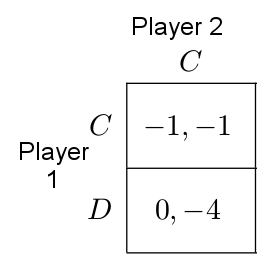
\includegraphics[width=5cm]{figures/ExamplePartialGrid1.png}
  \caption{Player 1's best response in the Prisoner's Dilemma, assuming Player 2 cooperates with Player 1}
  \label{fig:NashCol1}
\end{figure}

In Figure \ref{fig:NashCol1}, it is trivial to find the utility-maximizing strategy. In this case, the best response to player 2's cooperation is for player 1 to defect and accuse their partner: 1 year in prison or no time in prison. These steps are repeated for each of player 2's possible strategies.
\begin{figure}[H]
  \centering
  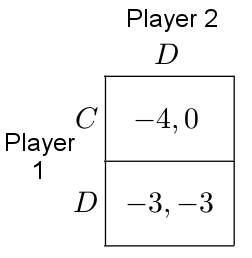
\includegraphics[width=5cm]{figures/ExamplePartialGrid2.png}
  \caption{Player 1's best response in the Prisoner's Dilemma, assuming Player 2 will defect against Player 1}
  \label{fig:NashCol2}
\end{figure}
So, assuming player 2 will defect to the police, player 1's best response is to defect as well: 3 years in prison or 4 years in prison. Since the best response is the same for all of player 2's strategies, this player will always choose this option. Using the same process for player 2 returns the same best response.

Thus, the Nash equilibrium is that both prisoners will defect, and both will get 3 years in prison. 

\begin{proof}
  Let $G=(N, A, u)$ be a normal-form game. $N = \{n_1, n_2\}$ is the set of players in the game. $A=A_1\times A_2$ is the set of actions in the game, where $A_1=\{c_1, d_1\}$ is the set of actions available to player 1, and $A_2=\{c_2, d_2\}$ is the set of actions available to player 2. Therefore, $A=\{(c_1, c_2), (c_1, d_2), (d_1, c_2), (d_1, d_2)\}$. The utility function $u=(u_1, u_2)$. $u_1=(c_1, c_2)\mapsto -1, (c_1, d_2)\mapsto -4, (d_1, c_2)\mapsto 0, (d_1, d_2)\mapsto -3$, and $u_2=(c_1, c_2)\mapsto -1, (c_1, d_2)\mapsto 0, (d_1, c_2)\mapsto -4, (d_1, d_2)\mapsto -3$.\\

  Let $s^*_1$ be a mixed strategy for $n_1$ where $n_1$ chooses action $d_1$. Since there are only two other players, the set of strategy profiles disjoint from $s_1$ is the same as $s_2$, the set of strategy profiles for $n_2$. Thus, $n_1$ has $s^*_1$ as a best response to $s_2$ if $u_1(s^*_1, s_2)\ge u_1(s_i, s_2)$ for all possible actions $s_i\in A_1$ and all strategies in $s_2$.\\
  
  $u_1(d_1, c_2)\ge u_1(c_1, c_2) \Rightarrow 0\ge -1$\\
  
  $u_1(d_1, c_2)\ge u_1(d_1, c_2) \Rightarrow 0\ge 0$\\

  $u_1(d_1, d_2)\ge u_1(c_1, d_2) \Rightarrow -3\ge -4$\\

  $u_1(d_1, d_2)\ge u_1(d_1, d_2) \Rightarrow -3\ge -3$\\

  $s^*_1$ is greater than or equal to all possible actions in $A_1$ and for all strategies in $s_2$. Thus, $s^*_1=d_1$ is the best response for player $n_1$.\\

  Let $s^*_2$ be a mixed strategy for $n_2$ where $n_2$ chooses action $d_2$. Since there are only two other players, the set of strategy profiles disjoint from $s_2$ is the same as $s_1$, the set of strategy profiles for $n_1$. Thus, $n_2$ has $s^*_2$ as a best response to $s_1$ if $u_2(s^*_2, s_1)\ge u_2(s_i, s_1)$ for all possible actions $s_i\in A_2$ and all strategies in $s_1$.\\
  
  $u_1(c_1, d_2)\ge u_1(c_1, c_2) \Rightarrow 0\ge -1$\\

  $u_1(c_1, d_2)\ge u_1(c_1, d_2) \Rightarrow 0\ge 0$\\

  $u_1(d_1, d_2)\ge u_1(d_1, c_2) \Rightarrow -3\ge -4$\\

  $u_1(d_1, d_2)\ge u_1(d_1, d_2) \Rightarrow -3\ge -3$\\

  $s^*_2$ is greater than or equal to all possible actions in $A_2$ and for all strategies in $s_1$. Thus, $s^*_2=d_2$ is the best response for player $n_1$. A strategy set $(s_1,\dots ,s_n)$ is a Nash equilibrium if $s_i$ is the best response for all players $i$. Therefore, the strategy profile $(d_1, d_2)$ is a Nash equilibrium for game $G$.
\end{proof}

Not all games have a Nash equilibrium; take the normal-form representation of rock-paper-scissors, for instance. Assume that the utility function award players 1 point for winning the game, -1 point for losing the game, and 0 points for a draw. We will position Player 1 be on the left side of the matrix, and Player 2 be on the top of the matrix.
\begin{figure}[H]
  \centering
  \begin{tabular}{r r | c | c | c |}
    &\multicolumn{1}{c}{}&\multicolumn{1}{c}{}&\multicolumn{1}{c}{Player 2}&\multicolumn{1}{c}{}\\
    Rock-Paper-Scissors &\multicolumn{1}{c}{}&\multicolumn{1}{c}{Rock}&\multicolumn{1}{c}{Paper}&\multicolumn{1}{c}{Scissors} \\ \cline{3-5}
    & Rock & (0, 0) & (-1, 1) & (1, -1) \\ \cline{3-5}
    Player 1 & Paper & (1, -1) & (0, 0) & (-1, 1) \\ \cline{3-5}
    & Scissors & (-1, 1) & (1, -1) & (0, 0) \\ \cline{3-5}
  \end{tabular}
  \caption{The normal-form representation of the game Rock-Paper-Scissors}
  \label{fig:RPS}
\end{figure}

Every row and every column in this Figure \ref{fig:RPS} has the same three results, and none of the choices is a winning strategy for more than one situation. Rock may beat Scissors, but it loses to Paper. If the Nash equilibrium of Player 1 is investigated, each possible action by Player 2 results in a different best response for Player 1. Thus, there can be no equilibrium.

\subsection{Non-Simultaneous Games}

It is important to recognize in these two examples that both players are making their choice simultaneously. Games without simultaneous actions are not so easily expressed in normal form. For example, take a game of tic-tac-toe. For simplicity, assume that the game is played with a 2x2 board instead of a 3x3 board. Assume the utility function award players 1 point for winning the game, -1 point for losing the game, and 0 points for a draw. Let UL be a piece in the upper left square, UR the upper right square, LL the lower left square, and LR the lower right square. We position Player 1 be on the left side of the matrix, and Player 2 be on the top of the matrix. Assume Player 1 has the first turn.\\
\begin{figure}[H]
  \centering
  \begin{tabular}{r r | c | c | c | c |}
    &\multicolumn{1}{c}{}&\multicolumn{1}{c}{}&\multicolumn{1}{c}{Player 2}&\multicolumn{1}{c}{}\\
    \multicolumn{1}{c}{2x2 tic-tac-toe}&\multicolumn{1}{c}{}&\multicolumn{1}{c}{UL}&
    \multicolumn{1}{c}{UR}&\multicolumn{1}{c}{LL}&\multicolumn{1}{c}{LR}\\ \cline{3-6}
    & UL & x & (0, 0) & (0, 0) & (0, 0) \\ \cline{3-6}
    Player 1 & UR & (0, 0) & x & (0, 0) & (0, 0) \\ \cline{3-6}
    & LL & (0, 0) & (0, 0) & x & (0, 0) \\ \cline{3-6}
    & LR & (0, 0) & (0, 0) & (0, 0) & x \\ \cline{3-6}
  \end{tabular}
  \caption{The first two moves of a tic-tac-toe variant using a 2x2 game board.}
  \label{fig:2x2TTT}
\end{figure}

Figure \ref{fig:2x2TTT} shows the normal form for the first two moves of this game. Since each player has only placed a single piece, neither one has won yet; thus, the utility for each space is (0,0). There are four spaces in the matrix marked with an 'x'. These spaces are infeasible; it is against the rules for someone to play on the same square as someone else. Both players have made their first move, and it is Player 1's turn once again.\\
\begin{figure}[H]
  \centering
  \begin{tabular}{r r | c | c | c | c |}
    &\multicolumn{1}{c}{}&\multicolumn{1}{c}{}&\multicolumn{1}{c}{Player 2}&\multicolumn{1}{c}{}\\
    \multicolumn{1}{c}{2x2 tic-tac-toe}&\multicolumn{1}{c}{}&\multicolumn{1}{c}{UL}&
    \multicolumn{1}{c}{UR}&\multicolumn{1}{c}{LL}&\multicolumn{1}{c}{LR}\\ \cline{3-6}
    & (UL, UR) & x & x & (1, -1) & (1, -1) \\ \cline{3-6}
    & (UL, LL) & x & (1, -1) & x & (1, -1) \\ \cline{3-6}
    & (UL, LR) & x & (1, -1) & (1, -1) & x \\ \cline{3-6}
    & (UR, UL) & x & x & (1, -1) & (1, -1) \\ \cline{3-6}
    & (UR, LL) & (1, -1) & x & x & (1, -1) \\ \cline{3-6}
    Player 1 & (UR, LR) & (1, -1) & x & (1, -1) & x \\ \cline{3-6}
    & (LL, UL) & x & (1, -1) & x & (1, -1) \\ \cline{3-6}
    & (LL, UR) & (1, -1) & x & x & (1, -1) \\ \cline{3-6}
    & (LL, LR) & (1, -1) & (1, -1) & x & x \\ \cline{3-6}
    & (LR, UL) & x & (1, -1) & (1, -1) & x \\ \cline{3-6}
    & (LR, UR) & (1, -1) & x & (1, -1) & x \\ \cline{3-6}
    & (LR, LL) & (1, -1) & (1, -1) & x & x \\ \cline{3-6}
  \end{tabular}
  \caption{The full normal form representation of a 2x2 tic-tac-toe variant}
  \label{fig:full2x2TTT}
\end{figure}

Since the game board was shrunk for this example, the game ends with Player 1 always winning on their second turn. But even in this simplified game, the normal form in Figure \ref{fig:full2x2TTT} quickly becomes convoluted and cluttered. While the infeasible actions are fairly self-evident in Figure \ref{fig:2x2TTT}, illegal moves are less obvious in Figure \ref{fig:full2x2TTT}.
\begin{figure}[H]
  \centering
  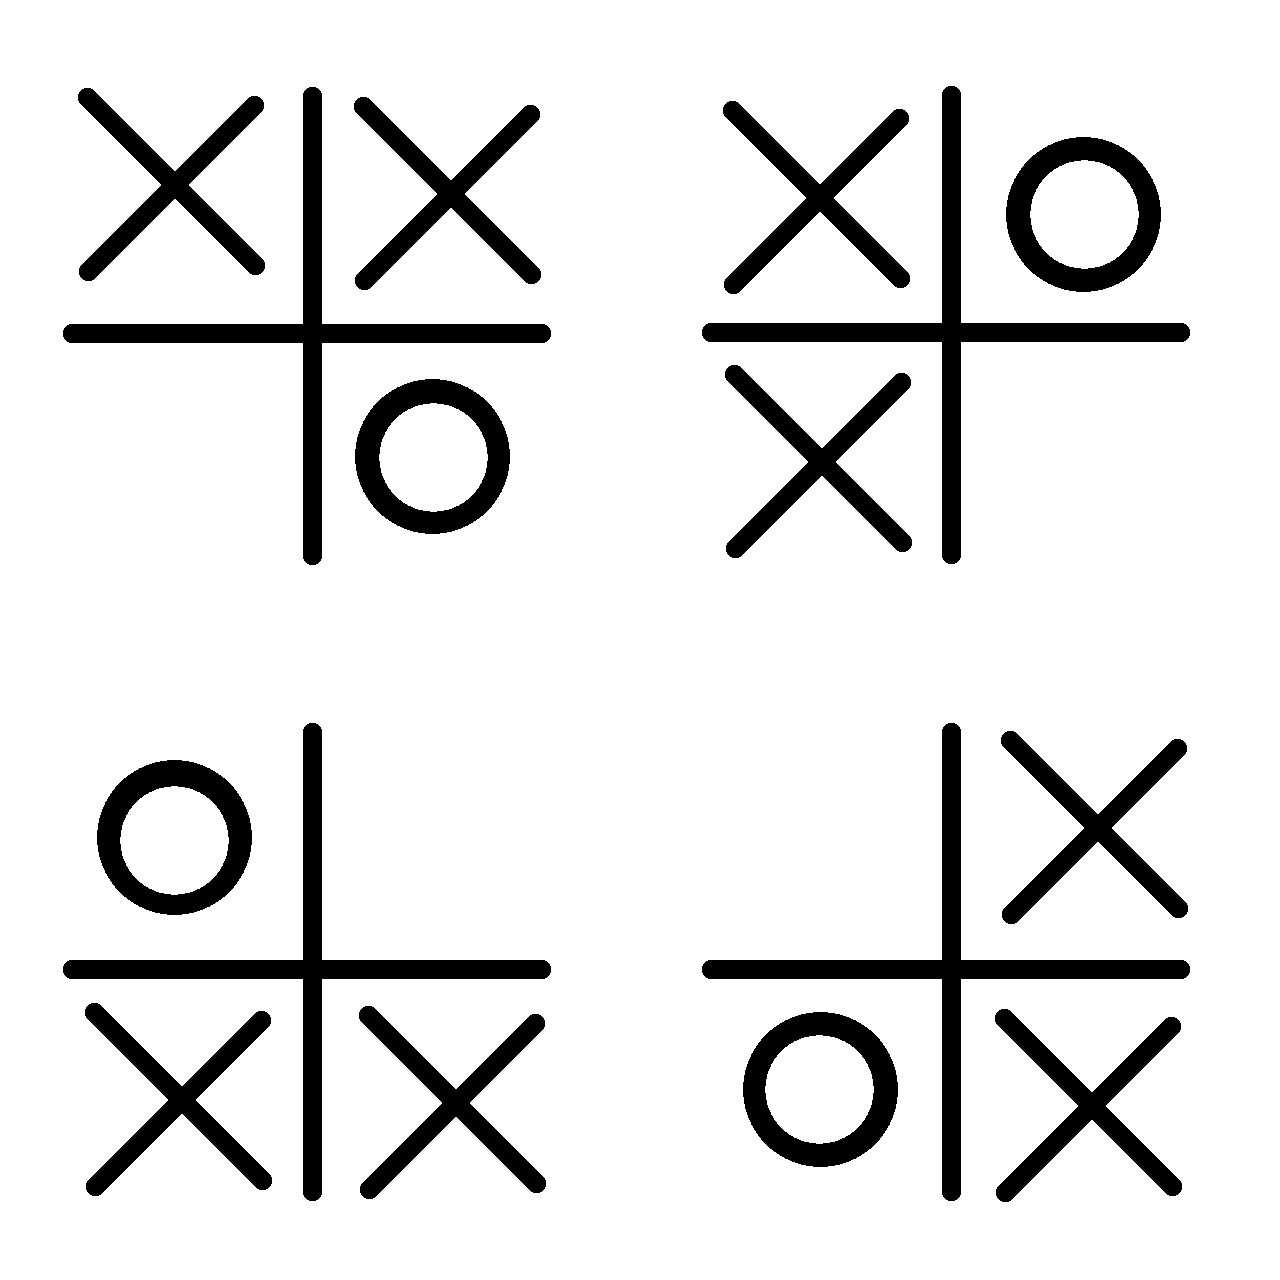
\includegraphics[width=6cm]{figures/TTTRotation.png}
  \caption{Rotational symmetry in a 2x2 tic-tac-toe game}
  \label{fig:2x2TTTRotation}
\end{figure}
There are also repeated game configurations: the outcome \{(UL, UR), (LR)\} is rotationally symmetrical to \{(LL, UL), (UR)\}, \{(LR, LL), (UL)\}, and \{(UR, LR), (LL)\}, as is evident in Figure \ref{fig:2x2TTTRotation}. Furthermore, the game \{(UL, UR), (LR)\} is identical to \{(UR, UL), (LR)\}. With so many extraneous spaces in the normal-form representation, it is no longer sufficient to represent player choices for games with sequential actions. Instead, these games are better represented in extensive-form trees.\\

\section{Extensive Form Trees}
In a turn-based, or extensive-form game, players do not make simultaneous actions. This leads to larger variety in gameplay. A simultaneous game like Rock-Paper-Scissors relies on chance; tic-tac-toe relies on players anticipating the future choices their opponents will make. There are two types of extensive-form games: perfect-information and imperfect-information. In perfect-information games, all players know which turn of the game they are at, while imperfect-information games have turns that are indistinguishable from others based on information available to the player. We will be dealing with perfect-information games.\\

\begin{define}
  A finite perfect information game in extensive form is a tuple $G = (N, A, H, Z, \chi, \rho, \sigma, u)$ where:
  \begin{itemize}
  \item $N$ is a set of n players;
  \item $A$ is a single set of actions;
  \item $H$ is a set of non-terminal, choice nodes;
  \item $Z$ is a set of terminal nodes, disjoint from $H$;
  \item $\chi: H\mapsto 2^A$ is the action function, mapping a set of possible actions to each choice node;
  \item $\rho: H\mapsto N$ is the player function, mapping to each non-terminal node a player who makes an action at said node;
  \item $\sigma: H\times A\mapsto H\bigcup Z$ is the successor function, mapping a choice node and an action to a new choice or terminal node. $\forall h_1, h_2\in H$ and $a_1, a_2\in A$, if $\sigma(h_1, a_1)=\sigma(h_2, a_2)$, then $h_1=h_2$ and $a_1=a_2$;
  \item $u=(u_1,...,u_n)$, where $u_i:Z\mapsto \mathbb{R}$ is a real-valued utility function for each player $i$ on a terminal node $Z$ \cite{shoh09}.
  \end{itemize}
\end{define}

As in the normal-form definition, there are $n$ players in the game, contained in the set $N$. $A$ is the set of all actions that could be performed in the course of the game. The set $H$ contains any and all choices or turns that do not end the game, while $Z$ contains all choices or turns that do end the game. The mapping function $\chi$ allocates the choices in $H$ a subset of possible actions from the set $A$, and the mapping function $\rho$ assigns these choices to the players who make them. $\sigma$ takes the actions assigned with $\chi$ and uses them to connect various nodes in $H$ and $Z$ together, creating the sequence of events in the game. Finally, $u$ contains utility functions for each player that determines their individual utility at each of the terminal nodes in $Z$.\\

\begin{figure}[H]
  \centering
  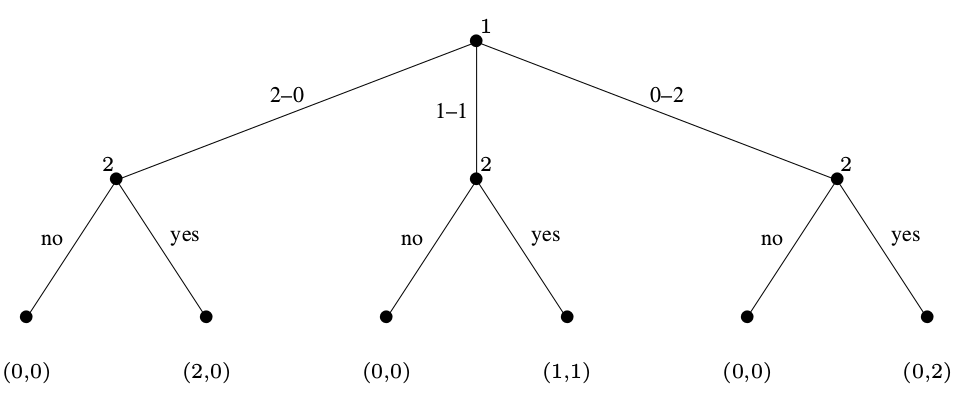
\includegraphics[width=10cm]{figures/ExampleTree.png}
  \caption{An extensive-form tree for The Sharing Game \cite{shoh09}}
  \label{fig:sharingTree}
\end{figure}

An example of the extensive-form tree can be seen in Figure \ref{fig:sharingTree}. The six leaf nodes of this tree are the elements of the set $Z$, while the other nodes are contained in $H$. The $H$ nodes are labeled either 1 or 2, denoting from the $\rho$ function which player is making the choice at that node. The $Z$ nodes each have a pair, denoting the utility each player will gain if the game ends in that particular way. The actions $A$ are denoted in the lines connecting the nodes together. In this game, the three actions from the root node are the methods of sharing 2 presents between 2 people. The second player, once the first player has distributed the presents in a particular way, chooses whether to accept the distribution or not.\\

To explore this definition, return to the game of tic-tac-toe. Let $N={N_1, N_2}$ be the set of players in the game. In this game, $A$ is the set of playing on one of the open spaces on the board; for the first move of the game, $A$ is the set of 9 open spaces on the board, for the second move, $A$ is the set of the remaining 8 spaces. For a game of tic-tac-toe, $H$ contains configuration of the board where neither player has three in a row and there are still open squares on the board. $Z$, on the other hand, contains the board configurations where one player has three in a row or all spaces have been claimed. For tic-tac-toe, the $\chi$ function removes illegal actions from a node, which in tic-tac-toe would be playing on an occupied square. Thus, the $\chi$ function leaves the choice nodes at each successive turn with fewer and fewer available actions. Since there are only two players, the $\rho$ function alternates between players after each action.

\begin{figure}[H]
  \centering
  
\includegraphics[width=16cm]{figures/TTTExtTree.png}
  \caption{The extensive-form representation of a 2x2 tic-tac-toe game}
  \label{fig:2x2TTTExtForm}
\end{figure}

Figure \ref{fig:2x2TTTExtForm} shows the extensive-form version of the 2x2 tic-tac-toe variant in Figure \ref{fig:full2x2TTT}. In comparison to the normal-form representation, the extensive-form tree can convey the sequence and flow of the game more clearly. Since the $\chi$ function of an extensive-form game only maps possible actions, the tree does not have the same infeasible nodes as the normal-form representation. This tree has the same issues of rotational symmetry as in the normal form, but in this particular example, the four subtrees connected to the root are all rotationally symmetrical to each other.

\subsection{Equilibria in Extensive-Form}
Nash equilibria can be found in extensive-form games as well, and are defined the same as in normal-form games. However, a pure strategy in an extensive-form game requires the player's strategy to contain the decision at every choice node, even if that node is unreachable by other choices in said strategy.\\
\begin{define}
  Let $G = (N, A, H, Z, \chi, \rho, \sigma, u)$ be a perfect-information extensive-form game. The pure strategies of player $i$ consist of the Cartesian product $\Pi_{h\in H, \rho(h)=i}\chi(h)$ \cite{shoh09}.
\end{define}
Given a perfect-information game, a player's pure strategy is the set of choices mapped by $\chi$ from each of that player's choice nodes $h$. It is a complete specification of the choices that a player determines they should make \cite{shoh09}. Since the actions of all other players are known in an extensive-form game, it is not necessary to introduce probabilities to determine a Nash equilibrium. Instead, Nash equilibria can be found using backwards induction.
%\begin{algorithm}
%  \caption{Backwards Induction \cite{shoh09}}
%  \begin{algorithmic}[1]
%    \Procedure {BackwardInduction}{node $h$}
%    \If{$h\in Z$}
%    \State Return $u(h)$
%    \Comment If $h$ is a leaf node, return the utility of that outcome
%    \EndIf
%    \For{$a\in\chi(h)$}
%    \State $util\_at\_child \gets BackwardInduction(\sigma(h, a))$
%    \Comment Recursively check each child of $h$
%    \If{$util\_at\_child_{\rho(h)}>best\_util_{\rho(h)}$}
%    \State $best\_util\gets util\_at\_child$\\
%    \Comment $best\_util$ holds the utility which is maximized for the player $\rho(h)$
%    \EndIf
%    \EndFor
%    \State Return $best\_util$
%    \EndProcedure
%  \end{algorithmic}
%\end{algorithm}

\lstset{language=pseudocode, label={lst:BackwInd}, caption={The Backward Induction algorithm for extensive-form game trees \cite{shoh09}.}}
\begin{lstlisting}[language=pseudocode]
  Procedure BackwardInduction(node h)
  if(h in Z)
      return u(h)
      //If h is a leaf node, return the utility of that outcome
  end if
  for(a in %*$\chi$*(h))
      util_at_child = BackwardInduction(%*$\sigma(h, a)$*)
      //Recursively check each child of h
      if(util_at_child%*$_{\rho(h)}$* > best_util%*$_{\rho(h)}$*)
          best_util = util_at_child
          //best_util holds the node which maximizes the utility of player %*$\rho$*(h)
      end if
  end for
  return best_util
  end Procedure
\end{lstlisting}

Backwards induction determines a dominant strategy for a particular game. The algorithm's base case is at line 2, where $h$ is in the set of terminal nodes in $Z$, or the leaves of the extensive-form tree. At these leaves the game is over, and the utility of that outcome is returned by the algorithm. When the node in question is not a terminal node, the algorithm checks the utility of each of that node's children at line 5. Since the child nodes may have their own children, line 6 recursively checks each child and gets the utility of that node. In lines 7 and 8, the backwards induction algorithm determines which node provides the player at node $h$ (as determined by the mapping function $\rho$) the maximum amount of utility. This node is returned in line 12.\\

\begin{figure}[H]
  \centering
  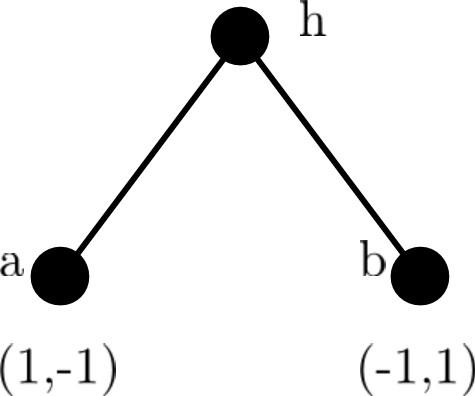
\includegraphics[width=4cm]{figures/ExampleBackwardInduction.png}
  \caption{A small extensive-form tree. The outcome is dependant on the player mapped by $\rho(h)$.}
  \label{fig:BackwardInduction}
\end{figure}
For example, examine the extensive-form tree for a two-player game in Figure \ref{fig:BackwardInduction}. with a root and two child, terminal nodes. At the leaf node $a$, player 1 has positive utility while player 2 has negative utility; at leaf node $b$, player 2 has positive utility and player 1 has negative utility. Since both players are utility-maximizing agents, the choice of the outcome is determined by whichever player happens to be making the decision, as mapped by $\rho(h)$. Suppose that Figure \ref{fig:BackwardInduction} is a subtree in a larger game. Further suppose that, in this larger game, the subtree in Figure \ref{fig:BackwardInduction} always has player 1 making the choice at node $h$. Given this scenario, player 1 will always perform the action that gets them to node $a$. Thus, node $h$ can be replaced by $a$, with $b$ being removed from the tree entirely, and the rest of the game will be unchanged. If the entire tree for a game is mapped out, then this process can be repeated all the way up to a root node; at that point, .
%\chapter{Extensive Form Games}
%\section{Game Theory}
%\subsection{Game Trees}
\chapter{Fuzzy Logic}
\section{Fuzzy Sets}
\section{Fuzzy Constraint Satisfaction Problem}
\chapter{Video Game AI}
\section{Fuzzy-State Machines}
\chapter{Description of Software}
\section{AI Model}
\section{Pygame}
\chapter{Future Work}
%\input{chapters/chapter3}
%\input{chapters/chapter4}
%\input{chapters/chapter5}
%\input{chapters/chapter6}
%\input{chapters/chapter7}
%\input{conclusion}

%%%%%%%%%%%%%%%%%%%%%%%%%%%%%%%%%%%%%%%%%%%%%%%%%%%%%%%
%
%  This section starts the back matter. The back matter includes appendices, indicies, and the
%  bibliography
%
%%%%%%%%%%%%%%%%%%%%%%%%%%%%%%%%%%%%%%%%%%%%%%%%%%%%%%%

\backmatter

%\input{appendices/math}
%\input{appendices/java}
%\input{appendices/cpp}
%\input{appendices/afterword}

%%%%%%%%%%%%%%%%%%%%%%%%%%%%%%%%%%%%%%%%%%%%%%%%%%%%%%%
%
%  This section would be used if you are not using BibTeX. Look at Kopka and Daly for how to
%  format a bibliography manually as well as how to use BibTeX.
%
%%%%%%%%%%%%%%%%%%%%%%%%%%%%%%%%%%%%%%%%%%%%%%%%%%%%%%%

%\begin{thebibliography}{99}
%\bibitem{}
%\bibitem{}
%\end{thebibliography}

%%%%%%%%%%%%%%%%%%%%%%%%%%%%%%%%%%%%%%%%%%%%%%%%%%%%%%%
%
%  We used BibTeX to generate a Bibliography. I would recommend this method. However, it is
%  not required.
%
%%%%%%%%%%%%%%%%%%%%%%%%%%%%%%%%%%%%%%%%%%%%%%%%%%%%%%%

\renewcommand\bibname{References} % changes the name of the Bibliography

\nocite{*}% This command forces all the bibliography references to be printed -- not just 
          % those that were explicitly cited in the text.  If you comment this out, the bibliography
          % will only include cited references.
\ifthenelse{\boolean{woosterchicago}}{
\bibliographystyle{woosterchicago}}{\ifthenelse{\boolean{achemso}}{
\bibliographystyle{achemso}}{\bibliographystyle{plainnat}}}
% if you have used the woosterchicago class option then your references and citations will be in Chicago format. If you have used the achemso class option then your references and citations will be in the American Chemical Society format. If you do not specify a citation format then the default Wooster format will be used.
\bibliography{references} % load our Bibliography file

%%%%%%%%%%%%%%%%%%%%%%%%%%%%%%%%%%%%%%%%%%%%%%%%%%%%%%%
%
%                                                                Index
%
%  Uncomment the lines below to include an index. To get an index you must put 
%  \index{index text} after any words that you want to appear in the index.
%  Subentries are entered as \index{index text!subentry text}. You must also run the
%  makeindex program to generate the index files that LaTeX uses. The PCs are set to run
%  makeindex automatically.
%
%%%%%%%%%%%%%%%%%%%%%%%%%%%%%%%%%%%%%%%%%%%%%%%%%%%%%%%

\ifthenelse{\boolean{index}}{
\cleardoublepage
\phantomsection
\addcontentsline{toc}{chapter}{Index}
\printindex}{}

%%%%%%%%%%%%%%%%%%%%%%%%%%%%%%%%%%%%%%%%%%%%%%%%%%%%%%%
%
%                                                                Colophon
%
%  A Colophon is a section of a printed document that acknowledges the designers and printers of the work.
% The colophon also includes information about the fonts and paper used in the printing. It is not required 
% for your IS and can be commented out.
%
%%%%%%%%%%%%%%%%%%%%%%%%%%%%%%%%%%%%%%%%%%%%%%%%%%%%%%%

\ifthenelse{\boolean{colophon}}{
\begin{colophon}
This Independent Study was designed by Dr. Jon Breitenbucher.\newline
It was edited and set into type in Wooster, Ohio,\newline
using the \ifthenelse{\boolean{xetex}}{\XeTeX\ typesetting system designed by Jonathan Kew}{\LaTeX\ typesetting system designed by Leslie Lamport}\newline
and based on the original \TeX\ system of Donald Knuth.\newline
It was printed and bound by Office Services at The College of Wooster.

The text face is Adobe Garamond Pro, designed by Robert Slimbach.\newline
This is the Opentype version distributed by Adobe Systems\newline
and purchased as part of the Adobe Type Classics for Learning.

The paper is standard laser copier paper and not of archival quality.
\end{colophon}}{}
\clearpage\thispagestyle{empty}\null\clearpage
\end{document}